\documentclass[conference]{IEEEtran}
\IEEEoverridecommandlockouts
\usepackage{cite}
\usepackage{amsmath,amssymb,amsfonts}
\usepackage{graphicx}
\usepackage{textcomp}
\usepackage{xcolor}
\usepackage{booktabs}
\usepackage{multirow}
\usepackage{tikz}
\usetikzlibrary{arrows.meta,positioning}
\usepackage{pgfplots}
\pgfplotsset{compat=1.17}
\usepackage{url}
\usepackage{stfloats}

\def\BibTeX{{\rm B\kern-.05em{\sc i\kern-.025em b}\kern-.08em
    T\kern-.1667em\lower.7ex\hbox{E}\kern-.125emX}}

\begin{document}

\title{A Genetic Algorithm Approach to Automated Room, Faculty, and Class\\ Scheduling Optimization for a University Department}

\author{
\IEEEauthorblockN{Marven E. Jabian}
\IEEEauthorblockA{Department of Electrical Engineering\\ College of Engineering \\ Mindanao State University -- Iligan Institute of Technology \\ Iligan City, Philippines \\ marven.jabian@g.msuiit.edu.ph}
\and
\IEEEauthorblockN{Irish Mae Lariosa, Lemuel John Tabada, Mark Aron Verano, Mara Mae Sabate, Jeryl Wayco}
\IEEEauthorblockA{Department of Electrical Engineering\\ College of Engineering \\ Mindanao State University -- Iligan Institute of Technology \\ Iligan City, Philippines}
}

\maketitle

\begin{abstract}
Manually building a conflict-free semester schedule that assigns rooms, time slots, and faculty to every lecture and laboratory section of an academic department is a combinatorial constraint-satisfaction problem that grows quickly intractable by hand as the number of rooms, subjects, and faculty increases. This paper presents the design and preliminary evaluation of a genetic algorithm (GA)-based room, faculty, and class scheduling optimization system, developed and deployed as a web application for the Department of Electrical Engineering (DEE), Mindanao State University -- Iligan Institute of Technology (MSU-IIT). The system encodes the scheduling problem as a permutation of scheduling tasks, decodes each candidate ordering through a deterministic, hard-constraint-respecting greedy placement procedure, and evolves the population using tournament selection, order crossover (OX), swap mutation, and elitism, guided by a multi-objective fitness function that rewards full session placement, tight room utilization, laboratory time-window compliance, reduced Friday sessions, and protected faculty break periods. Genetic algorithm parameters (population size, generation budget, and time budget) auto-scale to problem complexity, requiring no manual tuning per semester. We evaluate the system through controlled synthetic benchmarks -- executing the deployed optimizer's own code across four problem scales, each compared against a single-pass greedy-only baseline -- and through field usage-log records collected during development testing of the deployed application. Across 40 controlled trials, the GA matched the greedy baseline's session-placement rate exactly in every trial while consistently achieving higher fitness through its soft-objective refinements (tighter room utilization, fewer late-laboratory and Friday sessions, more preserved faculty breaks), and field usage-log records corroborate reliable, fully conflict-free scheduling at realistic departmental scale; computation stayed within a few seconds even at the largest scale tested, though we also observe and report a measurable time-budget overshoot at that scale from the algorithm's once-per-generation termination check.
\end{abstract}

\begin{IEEEkeywords}
genetic algorithm, university timetabling, room scheduling, combinatorial optimization, permutation encoding, order crossover, multi-objective optimization
\end{IEEEkeywords}

\begin{table}[t]
\caption{Notation}
\label{tab:notation}
\centering
\small
\begin{tabular}{cl}
\toprule
Symbol & Meaning \\
\midrule
$R,\,F,\,D,\,T$ & Sets of rooms, faculty, days, time slots \\
$S,\,s_i$ & Set of scheduling tasks; the $i$-th task \\
$d_i,\,c_i,\,\tau_i$ & Task $s_i$'s duration (slots), class size, subject type \\
$Q_i$ & Faculty qualified/authorized to teach $s_i$ \\
$m,\,p$ & Number of rooms, number of faculty \\
$N_{\text{sched}}$ & Sessions successfully placed \\
$G_{\text{room}}$ & \emph{gapScore}: idle slots trapped inside used room-days \\
$A_{\text{room}}$ & Distinct room-days occupied at all \\
$N_{\text{lateLab}}$ & Laboratory sessions ending after 6:00 PM \\
$N_{\text{Fri}}$ & Sessions placed on Friday \\
$N_{\text{noBreak}}$ & Faculty with no protected break window free \\
$G_{\text{fac}}$ & \emph{facultyGapScore}: idle time in faculty daily schedules \\
$C$ & Computed problem-complexity score, Eq.~(2) \\
$k$ & Tournament selection size \\
\bottomrule
\end{tabular}
\end{table}

\section{Introduction}

Every academic term, an engineering department must assign every lecture and laboratory section to a room, a time slot, and a qualified instructor, while satisfying a web of hard institutional rules and softer scheduling preferences. At the Department of Electrical Engineering (DEE), College of Engineering, MSU-Iligan Institute of Technology, this task involves multiple concurrent degree programs and year levels, rooms shared with other departments under fixed usage quotas, subjects handled entirely by other colleges (\emph{External Assignment}), and faculty who must never be double-booked across any of the rooms they might be assigned to. Building such a schedule manually requires simultaneously tracking room capacity and type (lecture vs. laboratory), faculty availability, regular-student cohort conflicts (a student cannot attend two required courses at once), and softer preferences such as protecting faculty break periods and avoiding Friday sessions to support energy conservation. A single late change -- a new room, an added section, a faculty substitution -- can cascade into conflicts elsewhere that are typically discovered only through repeated manual re-checking.

This class of problem, the University Course Timetabling Problem (UCTP), is a well-studied NP-hard combinatorial optimization problem \cite{abdelhalim2016}. Exact solvers do not scale to realistic institutional sizes, which has motivated decades of metaheuristic research, with genetic algorithms (GAs) emerging as one of the most consistently effective and widely adopted approaches \cite{subang2024,yan2025}.

This paper describes a GA-based Room Scheduling Optimization System built for and deployed at the DEE. Rather than presenting only the system's features, this paper focuses specifically on its \emph{optimization method}: the chromosome encoding, the deterministic decoder that turns a candidate ordering into a concrete, hard-constraint-respecting timetable, the multi-objective fitness function, the genetic operators, and the complexity-adaptive parameter scaling that removes the need for per-semester manual tuning. We further report preliminary experimental results obtained by (1) extracting and executing the deployed optimizer's exact production code in a controlled, repeatable benchmark harness across four synthetic problem scales, each compared against a single-pass greedy-only baseline to isolate the genetic algorithm's contribution, and (2) real field usage-log telemetry collected while the deployed application was being tested during development.

The contributions of this paper are:
\begin{itemize}
\item A fully specified, nine-constraint hard-constraint model (Section III) and a six-term multi-objective fitness function (Section IV-C) for departmental room/faculty/class scheduling, including the exact weighting used in a deployed system.
\item A complexity-adaptive parameter-scaling formula (Section IV-E) that removes the need for per-semester manual tuning of population size, generation budget, and computation time.
\item A controlled benchmark that isolates the genetic algorithm's contribution from the underlying greedy constraint solver by comparing both against an identical decoder on the same problem instances, across four synthetic problem scales (Section V-A).
\item Preliminary results combining this controlled benchmark with real field usage-log telemetry from a deployed application (Section VI).
\end{itemize}

The remainder of this paper is organized as follows. Section II reviews related work on GA-based timetabling. Section III formalizes the scheduling problem addressed. Section IV details the proposed methodology: encoding, decoding, fitness function, genetic operators, and adaptive parameter scaling. Section V describes the experimental setup. Section VI presents and discusses preliminary results. Section VII concludes and outlines future work.

\section{Related Work}

The university course timetabling problem has been addressed with a wide range of metaheuristics, with genetic algorithms remaining among the most practical and effective for realistic, institution-scale instances.

Abdelhalim and El Khayat \cite{abdelhalim2016} proposed a Utilization-based Genetic Algorithm (UGA) that seeds its initial population with heuristically constructed, feasible-quality timetables and applies a weighted-sum fitness function balancing hard constraints (room and instructor availability) against soft preferences such as instructor scheduling preferences and room-utilization efficiency, validated on a real case study at the Faculty of Commerce, Alexandria University. Their results demonstrate that GA search seeded with heuristic solutions -- an approach this paper's system also adopts -- consistently produces feasible, well-utilized timetables for real institutional data.

More recent work has focused on improving GA convergence and solution quality specifically for course scheduling. Subang \emph{et al.} \cite{subang2024}, in a Philippine case study, implemented a dynamic GA-based course-scheduling framework using selection, crossover, and mutation operators and reported meaningful reductions in scheduling conflicts and improved resource utilization relative to manual scheduling. Yan and Deng \cite{yan2025} introduced an adaptive genetic algorithm -- combining simulated annealing with multi-strategy selection -- for computer-course scheduling under increasing educational-informatization demands, reporting measurable gains in both scheduling accuracy and computation time over baseline GA variants.

Because a class schedule is fundamentally an assignment problem over an ordering of tasks, permutation encoding is a natural representation for GA-based timetabling. Cicirello \cite{cicirello2023} surveyed and empirically analyzed the crossover and mutation operators developed for permutation-encoded evolutionary algorithms, including order crossover (OX) and swap mutation -- the two operators used by the system in this paper -- concluding that operator choice should be matched to the structural features of the specific permutation problem being solved.

Beyond the optimization algorithm, prior work has examined how such systems are delivered to end users. Ginting \emph{et al.} \cite{ginting2022} designed a web-based lecture-scheduling information system for the Faculty of Engineering and Science, Ibn Khaldun University, letting department staff generate and manage schedules through a browser-based interface rather than manual spreadsheets -- the delivery model this paper's system also adopts, packaging the optimizer behind a browser-based application usable without specialized software installation.

Genetic algorithms are not the only metaheuristic applied to educational timetabling. Ceschia \emph{et al.} \cite{ceschia2012sa} designed and experimentally tuned a simulated-annealing solver for the post-enrolment course timetabling problem, reporting new best-known results on standard public benchmark instances through careful neighborhood and cooling-schedule engineering rather than population-based search; the same authors' later survey \cite{ceschia2022survey} situates simulated annealing, tabu search, and constraint programming alongside genetic algorithms as the four metaheuristic families that dominate the educational-timetabling literature, and reports that no single family is uniformly best across all benchmark families -- practical performance depends heavily on how well an approach's neighborhood or operator structure matches a given institution's specific constraint mix. This motivates our choice of a GA whose genetic operators (Section IV-D) and greedy decoder (Section IV-B) are purpose-built around the DEE's specific constraint structure (paired lecture sessions, shared-room caps, multi-program cohort conflicts) rather than a generic timetabling formulation, and motivates benchmarking against simulated annealing and constraint programming on the same DEE-specific instances as future work (Section VII).

This paper differentiates itself from the above by (i) reporting the exact, fully specified multi-objective fitness function and complexity-adaptive parameter-scaling formulas used in a deployed system, (ii) evaluating the genetic algorithm against a greedy-only baseline decoded through the identical constraint-checking procedure, isolating the contribution of evolutionary search from the contribution of the constraint solver itself, and (iii) reporting field usage-log telemetry from real (development-stage) use of the deployed application alongside controlled synthetic benchmarks. Table \ref{tab:related} summarizes how this places relative to the closest prior systems reviewed above.

\begin{table}[t]
\caption{This System vs. Closest Prior GA-Based Timetabling Systems}
\label{tab:related}
\centering
\footnotesize
\begin{tabular}{p{1.15cm}p{1.55cm}p{1.5cm}p{2.5cm}}
\toprule
System & Encoding & Baseline compared? & Field data reported? \\
\midrule
UGA \cite{abdelhalim2016} & Direct, weighted-sum fitness & Not vs. non-GA & Case study only \\
\cite{subang2024} & GA (DEAP), operators unspecified & No & Simulation only \\
\cite{yan2025} & Adaptive GA + SA & Vs. baseline GA variants & Simulation only \\
\cite{ginting2022} & Greedy Best-First (non-GA) & N/A & Case study only \\
This work & Permutation, greedy decoder & Vs. greedy-only, same decoder & Field usage log + benchmark \\
\bottomrule
\end{tabular}
\end{table}

\section{Problem Formulation}

Let $R = \{r_1, \dots, r_m\}$ be the set of rooms, $F = \{f_1, \dots, f_p\}$ the set of faculty, $D = \{\text{Mon}, \dots, \text{Sun}\}$ the set of days, and $T = \{t_1, \dots, t_{27}\}$ the set of 30-minute time slots spanning 7:30 AM--9:00 PM. A scheduling \emph{task} $s_i \in S$ represents one class session (a single lecture/laboratory meeting, or one half of a paired 1.5-hour lecture session) requiring a contiguous block of $d_i$ slots, a class size $c_i$, a subject type $\tau_i \in \{\text{LEC}, \text{LAB}\}$, and an optional set of qualified faculty $Q_i \subseteq F$.

A feasible assignment maps every task $s_i$ to a tuple $(r, d, t) \in R \times D \times T$ (or a room-free tuple $(d,t)$ for an External-Assignment task) subject to the following \textbf{hard constraints}:

\begin{itemize}
\item[H1] \textbf{Room-type compatibility}: a room configured as LEC-only or LAB-only never hosts the other subject type.
\item[H2] \textbf{Capacity}: the assigned room's capacity must be $\geq c_i$.
\item[H3] \textbf{Room non-overlap}: no two tasks occupy the same room at overlapping slots on the same day.
\item[H4] \textbf{Faculty non-overlap}: no two tasks assigned to the same faculty member overlap in time, checked globally across every room.
\item[H5] \textbf{One session per day}: no subject instance is scheduled twice on the same day.
\item[H6] \textbf{Regular-student cohort non-overlap}: two required courses for the same degree program, year level, and block must never overlap, since one cohort of students must attend both.
\item[H7] \textbf{Sunday exclusion}: no task is scheduled on Sunday, except the two NSTP course codes conventionally held then.
\item[H8] \textbf{Shared-room usage cap}: a room shared with another department is never booked past an administrator-defined percentage of its weekly open slots.
\item[H9] \textbf{Paired-session synchrony}: a 3-unit lecture subject split into two 1.5-hour sessions must occupy the \emph{same} room and time slot on both days of a matched day-pair (Mon/Wed, Tue/Thu, or Fri/Sat), with a qualified faculty member free on both days.
\end{itemize}

Subject to H1--H9, the system optimizes six \textbf{soft objectives}, described formally in Section IV-C: (i) maximize the number of sessions successfully placed; (ii) maximize room-utilization density; (iii) keep laboratory sessions within a 7:30 AM--6:00 PM preferred window; (iv) minimize the number of sessions placed on Friday; (v) preserve a guaranteed break window for every faculty member; and (vi) minimize idle gaps in each faculty member's daily schedule. Objective (i) strictly dominates the rest: a schedule that places one more session is always preferred over any improvement to (ii)--(vi), reflecting that an unplaced class is a functional failure the department must resolve manually, while (ii)--(vi) are quality-of-life refinements.

\section{Proposed Methodology}

\subsection{Design Rationale: Indirect Encoding over Direct Assignment}
A GA for timetabling can encode a candidate solution \emph{directly} (each gene fixes a task's room, day, and start slot outright) or \emph{indirectly} (each gene only orders the tasks, and a separate decoder assigns room/day/slot deterministically). A direct encoding lets crossover and mutation act straightforwardly on the assignment itself, but almost every direct-encoded offspring produced by naive crossover violates at least one hard constraint (H1--H9), requiring a repair step or a heavily penalized fitness function to steer the search back toward feasibility -- and with nine interacting hard constraints, designing a repair procedure that is both fast and unbiased is itself a substantial undertaking. This system instead uses the indirect, permutation-based design of Cicirello's survey \cite{cicirello2023}: because \emph{every} permutation decodes, through the greedy procedure of Section IV-B, into a schedule that already satisfies H1--H9 by construction (infeasible placements are simply deferred to the unscheduled list rather than accepted), order crossover and swap mutation can recombine and perturb chromosomes freely without ever producing an invalid schedule, and the entire feasibility burden is concentrated in one well-tested decoder rather than distributed across every genetic operator. The trade-off is that the GA does not directly control \emph{where} a task lands, only the \emph{order} in which tasks compete for resources -- Section VI-A's finding that the heuristic-seeded baseline already matches the full GA's placement rate suggests that, for the problem scales tested, this indirection costs little in practice.

\subsection{Chromosome Encoding}
The system uses a \emph{permutation encoding}: a chromosome is an ordered list of scheduling tasks. Each subject in the roster is expanded into one or more tasks by \texttt{buildTasks()}: a non-split lecture or single-session laboratory becomes one \emph{single} task per weekly session; a 3-unit lecture eligible for the 1.5-hour split becomes one \emph{paired} task representing both weekly halves together (so the decoder can enforce H9 atomically); and a laboratory subject split across rooms for capacity reasons produces multiple independent single tasks, each with its own instance key so that its sections do not block each other off the same day. This expansion means the chromosome length (and hence the size of the search space, $|S|!$ over sequential placement decisions) reflects the actual number of scheduling decisions to be made, not just the number of subjects.

\subsection{Decoding Procedure}
Given an ordering (a chromosome), the system decodes it deterministically into a concrete schedule via a single left-to-right greedy pass (\texttt{runTrial}), maintaining per-room, per-faculty, and per-cohort occupancy grids that are updated as each task is placed:

\begin{enumerate}
\item For task $s_i$ in order, enumerate every $(r, d, t)$ triple satisfying H1--H9 given the \emph{already-placed} tasks before it (a room/day/faculty/cohort candidate search, restricted to rooms allowing the subject's type and rooms/days within their configured availability).
\item If no candidate exists, $s_i$ is recorded as \emph{unscheduled} with a diagnostic reason (room capacity, no continuous open block, faculty contention, or cohort contention -- determined by relaxing constraints one at a time until the blocking one is found), rather than aborting the whole decode.
\item Otherwise, candidates are ranked by the soft-objective heuristics of Section IV-C (laboratory time-window compliance first for LAB tasks, then Friday-avoidance, then room-load/adjacency packing, then minimal wasted capacity), and one is chosen: the top-ranked candidate with probability 0.7, or a uniformly random candidate among the top three otherwise. This controlled randomness lets different chromosome orderings explore genuinely different regions of the schedule space instead of always collapsing onto the same greedy choice.
\item The chosen slot is marked occupied in the relevant occupancy grids, and the loop continues to the next task.
\end{enumerate}

Because every task is checked against constraints H1--H9 \emph{before} being placed, the decoder produces a hard-constraint-respecting schedule by construction. A final safety-net pass (\texttt{validateAndSplitConflicts}) re-scans the completed assignment set for any residual room, faculty, or cohort overlap and pulls the offending sessions back out as unscheduled with an explicit conflict reason, so a decoding edge case never silently ships a double-booking.

For a single task, candidate enumeration is $O(m \cdot |D| \cdot |T|)$ (every room, every day, every start slot), so one full decode of an $|S|$-task chromosome is $O(|S| \cdot m \cdot |D| \cdot |T|)$; since $|D|$ and $|T|$ are fixed constants for a given institution (7 days, 27 half-hour slots), this reduces to $O(|S| \cdot m)$ per decode, matching the $|S| \cdot (1+\log_2(m{+}1))$ leading term of the complexity score $C$ in Eq.~(2). One full generation evaluates $\text{popSize}$ chromosomes, giving $O(\text{popSize} \cdot |S| \cdot m)$ work per generation -- the cost that Section VI-A's measured wall-clock overshoot at large problem scales is directly attributable to.

\subsection{Fitness Function}
Each decoded schedule is scored by a single scalar fitness function combining the placement count with five soft-objective penalty terms:
\begin{equation}
\begin{aligned}
\text{Fit} = \; & 100000 \cdot N_{\text{sched}} - 3 \cdot G_{\text{room}} - 6 \cdot A_{\text{room}} \\
& - 25 \cdot N_{\text{lateLab}} - 10 \cdot N_{\text{Fri}} - 15 \cdot N_{\text{noBreak}} - 4 \cdot G_{\text{fac}}
\end{aligned}
\label{eq:fitness}
\end{equation}
where $N_{\text{sched}}$ is the number of sessions successfully placed; $G_{\text{room}}$ (\emph{gapScore}) is the total number of idle slots trapped between the first and last booking of every room-day (a tight-packing measure); $A_{\text{room}}$ is the number of distinct room-days used at all (fewer, more concentrated room-days are preferred over many lightly-used ones); $N_{\text{lateLab}}$ is the count of laboratory sessions extending past the 6:00 PM preferred cutoff; $N_{\text{Fri}}$ is the count of sessions placed on Friday; $N_{\text{noBreak}}$ is the number of faculty members who were \emph{not} given at least one of the two protected break windows (10:30 AM--12:00 NN or 12:00 NN--1:30 PM) free across the whole week; and $G_{\text{fac}}$ (\emph{facultyGapScore}) is the total idle time trapped between each faculty member's first and last class of each day, summed over all faculty and days.

The coefficient of $N_{\text{sched}}$ (100{,}000) is chosen to dominate every other term by orders of magnitude: since each of the remaining terms is bounded by problem size (at most a few hundred for realistic departmental instances), no combination of soft-objective improvements can ever be preferred by the fitness function over placing one additional session. This encodes the placement-first, quality-second priority ordering of Section III directly into a single objective, avoiding the need for a Pareto-based multi-objective search while still balancing five secondary criteria.

\subsection{Genetic Operators}
The population evolves generation-to-generation using:

\textbf{Tournament selection.} A parent is chosen by drawing $k{=}3$ individuals uniformly at random from the evaluated population and returning the fittest of the three, applied independently to select each of the two parents for every child produced.

\textbf{Order crossover (OX).} Given parents $A$ and $B$, a random contiguous slice $[i,j]$ of $A$ is copied into the child at the same positions; the remaining positions are filled, in order, by scanning $B$ starting just after $j$ (wrapping around) and inserting each of $B$'s tasks that was not already copied from $A$. This always yields a valid permutation (no task duplicated or dropped) and preserves relative task ordering from both parents -- a property known to work well when, as here, the objective is sensitive to the sequence in which tasks compete for the same limited resources.

Table \ref{tab:ox} works a small example: with slice $[i,j]{=}[2,4]$ (0-indexed) copied from parent $A$ into the child at positions 2--4, the remaining positions (5, 6, 0, 1, in that wrap-around order) are filled by scanning $B$ starting at position 5 and inserting each task not already copied from $A$, skipping $c$, $d$, and $e$ where they recur in $B$.

\begin{table}[t]
\caption{Order Crossover (OX) Worked Example, $n{=}7$, slice $[2,4]$}
\label{tab:ox}
\centering
\small
\begin{tabular}{cccccccc}
\toprule
Position & 0 & 1 & 2 & 3 & 4 & 5 & 6 \\
\midrule
Parent $A$ & $a$ & $b$ & \bfseries c & \bfseries d & \bfseries e & $f$ & $g$ \\
Parent $B$ & $e$ & $g$ & $b$ & $f$ & $a$ & $c$ & $d$ \\
\midrule
Child & $f$ & $a$ & \bfseries c & \bfseries d & \bfseries e & $g$ & $b$ \\
\bottomrule
\end{tabular}
\end{table}

\textbf{Swap mutation.} With probability 0.25, a child undergoes 1--2 random pairwise position swaps -- a minimally disruptive perturbation standard for permutation-encoded GAs \cite{cicirello2023}, which nudges the search without destroying the structure crossover just assembled.

\textbf{Elitism.} The top $\lceil 0.08 \times \text{popSize} \rceil$ (minimum 2) individuals of each generation are copied unchanged into the next generation before the rest is filled by crossover and mutation, guaranteeing the best fitness found so far is never lost.

\subsection{Adaptive Parameter Scaling}
Rather than requiring per-semester manual tuning, the genetic algorithm's parameters scale automatically with a computed problem-complexity score:
\begin{equation}
C = |S| \cdot (1 + \log_2(m+1)) + 3p + n_{\text{subj}} + 1.5\,n_{\text{cohort}} + 4\,g_{\text{cohort}}
\label{eq:complexity}
\end{equation}
where $|S|$ is the total task (chromosome) length, $m$ is the room count, $p$ the faculty count, $n_{\text{subj}}$ the subject count, $n_{\text{cohort}}$ the number of tasks subject to a regular-student cohort constraint, and $g_{\text{cohort}}$ the number of distinct (cohort, block) occupancy grids in play. From $C$, the system derives:
\begin{align}
\text{popSize} &= \text{clamp}(\text{round}(1.5\,C),\ 20,\ 150) \\
\text{maxGen} &= \text{clamp}(\text{round}(2.2\,C),\ 25,\ 300) \\
\text{timeBudget (ms)} &= \text{clamp}(1500 + 40\,C,\ 1500,\ 6000)
\end{align}
so harder problems (more rooms widening the per-task search space via the $\log_2$ term, more faculty adding conflict constraints, more cohort groups adding combinatorial contention) automatically receive a larger population, a longer generation budget, and a longer wall-clock allowance, while small departmental instances terminate quickly. The initial population is seeded with one heuristic ordering (tasks sorted by descending duration then descending class size -- a most-constrained-first heuristic) plus $\text{popSize}{-}1$ random permutations, so the GA never starts from a worse position than a reasonable greedy baseline.

\subsection{Termination Criteria}
Evolution stops at the first of: (a) a \emph{perfect} generation is found -- every session placed, zero room-utilization gap, and zero late-laboratory sessions; or (b) the elapsed wall-clock time exceeds the adaptive time budget of Eq. (5). Termination is checked once per generation, so real elapsed time may exceed the nominal budget by up to one generation's decode cost; Section VI reports the resulting empirical wall-clock distribution.

\subsection{System Architecture}
The optimizer described above is embedded in a client-side web application (Fig. \ref{fig:pipeline}) with no server-side dependency for scheduling itself: Rooms, Subjects, and Faculty are managed through dedicated tabs (with CSV import/export), and a curriculum \emph{Prospectus} can be uploaded per degree program (CSV, or best-effort PDF parsing) and linked to a \emph{Target Semester}, which auto-populates that term's subjects and activates the regular-student cohort constraint (H6) for every affected program and year level simultaneously. Pressing \emph{Optimize} runs the algorithm of Sections IV-A--IV-F entirely in the browser and renders the result as a Room Timetable, a per-faculty schedule, a per-cohort regular-student schedule, and a flat list view, each printable and CSV-exportable; any task the decoder could not place is surfaced as a specific Room, Faculty, or Regular-Student conflict with the diagnostic reason identified during decoding (Section IV-B), rather than a generic failure. All scheduling data persists in the browser's local storage, so the system requires no backend database. An optional lightweight local server adds only anonymized usage tracking for app-functionality testing (Section V-B) and does not alter scheduling behavior.

Table \ref{tab:diagnostics} lists how an unplaced task's conflict type is determined: rather than reporting every failed task generically, the decoder relaxes constraints one at a time, from most to least restrictive, and reports the first relaxation that makes a candidate slot appear -- so a scheduler using the tool is told \emph{which} constraint to relax (e.g. ``add a bigger room'' vs. ``the assigned faculty member has no free slot'') rather than being left to re-derive the cause by hand.

\begin{table}[t]
\caption{Conflict Diagnosis: Checks Applied in Order (Single Tasks)}
\label{tab:diagnostics}
\centering
\footnotesize
\begin{tabular}{p{0.6cm}p{3.5cm}p{3.0cm}}
\toprule
\# & Check & Reported cause if this is the first to fail \\
\midrule
1 & Any room allows this subject type (H1) & No room hosts this subject type \\
2 & Some type-allowed room is large enough (H2) & No room seats this class size \\
3 & Some big-enough room has a continuous open block, any day (static availability) & No room has a long-enough open block \\
4 & ...and that block is not already booked by another session (H3) & Every big-enough room is already booked \\
5 & ...and booking it would stay within the shared-usage cap (H8) & Room(s) already at their usage cap \\
6 & ...and it falls on a day this subject instance is not already using (H5) & Only free on a day already used \\
7 & A slot exists respecting the cohort constraint (H6) with faculty ignored & Regular-student cohort conflict \\
8 & A slot exists respecting the faculty constraint (H4) with cohort ignored & Faculty double-booking \\
\bottomrule
\end{tabular}
\end{table}

\begin{figure}[t]
\centering
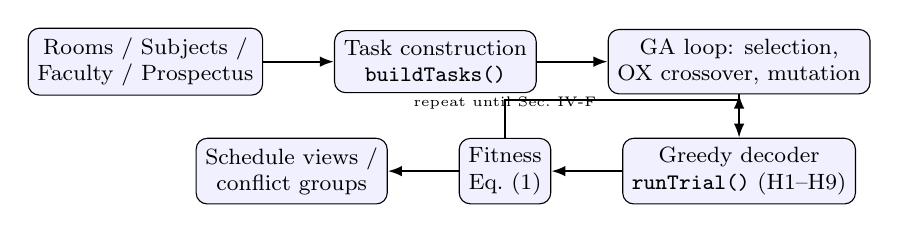
\begin{tikzpicture}[
  node distance=0.55cm and 0.9cm,
  box/.style={draw, rounded corners, align=center, minimum height=0.7cm, font=\footnotesize, fill=blue!6},
  arr/.style={-{Latex[length=1.8mm]}, thick}
]
\node[box] (data) {Rooms / Subjects /\\ Faculty / Prospectus};
\node[box, right=of data] (tasks) {Task construction\\ \texttt{buildTasks()}};
\node[box, right=of tasks] (ga) {GA loop: selection,\\ OX crossover, mutation};
\node[box, below=of ga] (decode) {Greedy decoder\\ \texttt{runTrial()} (H1--H9)};
\node[box, left=of decode] (fit) {Fitness\\ Eq.~(1)};
\node[box, left=of fit] (out) {Schedule views /\\ conflict groups};
\draw[arr] (data) -- (tasks);
\draw[arr] (tasks) -- (ga);
\draw[arr] (ga) -- (decode);
\draw[arr] (decode) -- (fit);
\draw[arr] (fit) -- node[above, font=\tiny]{repeat until Sec.~IV-F} ++(0,0.9) -| (ga);
\draw[arr] (fit) -- (out);
\end{tikzpicture}
\caption{Optimization pipeline: task construction, the GA loop (selection/crossover/mutation), the constraint-respecting greedy decoder, and fitness evaluation, iterating until the termination criteria of Section IV-F are met.}
\label{fig:pipeline}
\end{figure}

\section{Experimental Setup}

No public benchmark dataset matches this problem's exact institutional constraints (External Assignment subjects, shared-room usage caps, paired 1.5-hour lecture sessions, multi-program cohort conflict-checking), so we evaluate the system through two complementary sources of evidence.

\subsection{Controlled Synthetic Benchmark}
We extracted the optimizer's exact, unmodified production logic (task construction, the greedy decoder, the fitness function, and all genetic operators) from the deployed application's source and executed it directly in a Node.js harness, decoupled from the browser UI, so it could be driven programmatically at scale. Four synthetic problem scales were generated with a seeded pseudo-random generator for reproducibility, summarized in Table \ref{tab:scenarios}. For each scale, subjects were generated with a realistic LEC/LAB mix (65\%/35\%), realistic class sizes (20--45 students), a 50\% rate of 1.5-hour paired-session eligibility among lecture subjects, a 20\% rate of capacity-driven laboratory section splitting, and a small (5\%) proportion of External-Assignment subjects; faculty were assigned subjects round-robin.

\begin{table}[t]
\caption{Synthetic Benchmark Scenarios}
\label{tab:scenarios}
\centering
\begin{tabular}{lcccc}
\toprule
Scenario & Rooms & Subjects & Faculty & Sessions \\
\midrule
Small  & 3  & 10 & 3  & \input{tab_sessions_small.tex} \\
Medium & 5  & 25 & 6  & \input{tab_sessions_medium.tex} \\
Large  & 8  & 40 & 10 & \input{tab_sessions_large.tex} \\
XLarge & 10 & 55 & 14 & \input{tab_sessions_xlarge.tex} \\
\bottomrule
\end{tabular}
\end{table}

For each scenario we ran 10 independent trials (fresh random problem instance per trial, same scale parameters). Each trial ran the full genetic algorithm (\texttt{optimizeSchedule}) to its own natural termination (Section IV-F), and, on the identical problem instance, additionally decoded the single most-constrained-first heuristic ordering with no evolutionary search (a \emph{greedy-only baseline}, i.e. what generation 1 of a non-genetic greedy scheduler would produce) to isolate the contribution of the genetic algorithm from the contribution of the constraint-respecting decoder itself. We report, per scenario: session placement rate, generations to termination, wall-clock time, and the fitness/utilization sub-metrics of Eq. (\ref{eq:fitness}), each as mean $\pm$ standard deviation over the 10 trials. Because each trial decodes the same random problem instance with both methods, we additionally treat the 10 (GA, baseline) fitness pairs per scenario as a matched-pairs sample and report a paired $t$-test.

\subsection{Field Usage-Log Records}
Independently of the controlled benchmark, the deployed application logs anonymized usage telemetry -- including, for every optimizer run, the generation count reached, the auto-scaled population size, the room count, and the resulting scheduled/unscheduled session counts -- to support ongoing app-functionality testing. We report the aggregate of all optimizer runs logged during the system's development-testing period as an informal, real-world complement to the controlled benchmark. These records were \emph{not} collected as a designed experiment (problem sizes were whatever the tester happened to enter while exercising the application's features) and are reported as such.

\section{Results and Discussion}

\subsection{Synthetic Benchmark Results}
Table \ref{tab:results} summarizes the controlled benchmark. \input{tab_discussion_note.tex}

\begin{table*}[t]
\caption{Genetic Algorithm vs. Greedy-Only Baseline, by Scenario (mean $\pm$ std over 10 trials)}
\label{tab:results}
\centering
\small
\input{tab_results.tex}
\end{table*}

\input{results_narrative.tex}

\subsection{Convergence Behavior}
Fig. \ref{fig:convergence} plots the best-of-generation fitness for a representative Medium-scenario trial. \input{fig_convergence_note.tex}

\begin{figure}[t]
\centering
\input{fig_convergence.tex}
\caption{Best-of-generation fitness over the run for a representative Medium-scenario trial. The large initial jump reflects the dominance of the placement term in Eq. (\ref{eq:fitness}); subsequent generations refine room-utilization and faculty-preference sub-objectives.}
\label{fig:convergence}
\end{figure}

\subsection{Field Usage-Log Records}
\input{field_usage_note.tex}

\subsection{Threats to Validity}
Three limitations bound how far these preliminary results generalize. First, the synthetic benchmark's subject/room/faculty distributions are plausible approximations of DEE's actual course mix, not a sample of real historical scheduling data; the field usage-log records partially address this but reflect ad hoc developer testing, not a full semester's real roster. Second, the regular-student cohort constraint (H6) -- the most combinatorially demanding of the nine hard constraints -- was not exercised in the controlled benchmark and is left to future work (Section VII). Third, all trials were executed on a single machine; absolute wall-clock numbers will vary with hardware, though the \emph{relative} GA-vs-baseline comparison and the qualitative scaling trend are expected to hold.

\section{Conclusion and Future Work}

This paper presented the optimization core of a deployed Room Scheduling Optimization System for a university department: a permutation-encoded genetic algorithm with a deterministic, hard-constraint-respecting greedy decoder, a six-term multi-objective fitness function dominated by session placement, tournament selection, order crossover, swap mutation, elitism, and complexity-adaptive parameter scaling requiring no manual per-semester tuning. Preliminary evaluation through a controlled synthetic benchmark -- comparing the full genetic algorithm against a single-pass greedy-only baseline decoded through the identical constraint solver, across four problem scales and 40 trials -- together with field usage-log records from development testing of the deployed application, shows that the evolutionary search consistently and reliably improves the greedy baseline's schedule \emph{quality} (fitness) through its soft-objective terms, while matching its session-\emph{placement} rate exactly in every trial tested; computation stayed within a few seconds at every scale, though we also identified and report a measurable time-budget overshoot at the largest scale traceable to the algorithm's once-per-generation termination check.

Future work includes: (1) evaluating the system against a real, multi-program DEE semester roster exercising the regular-student cohort constraint (H6) at full combinatorial scale; (2) constructing tightly-constrained problem instances (little room/faculty slack) where the most-constrained-first heuristic is expected to under-perform, to isolate and quantify the genetic algorithm's contribution to \emph{placement feasibility} rather than schedule quality alone -- the present benchmark's heuristic-seeded baseline matched the full GA's placement rate in all 40 trials, so this remains an open question rather than a settled negative result; (3) checking the adaptive time budget \emph{within} a generation's decode-and-evaluate loop, not only between generations, to bound the measured wall-clock overshoot observed at the XLarge scale (Section VI-A); (4) a controlled ablation over individual fitness-term weights and genetic operator choices (e.g., partially-mapped or cycle crossover in place of OX) to quantify each design decision's marginal contribution; (5) benchmarking against alternative metaheuristics (simulated annealing, constraint programming) on the same problem instances; and (6) a post-deployment user study measuring the time DEE staff save relative to manual scheduling, and gathering structured feedback to refine the fitness function's weighting of soft objectives.

\section*{Acknowledgment}
The authors thank the Department of Electrical Engineering, MSU-Iligan Institute of Technology, for the scheduling requirements and data that shaped this system's design.

\begin{thebibliography}{00}
\bibitem{abdelhalim2016} E.~A. Abdelhalim and G.~A. El Khayat, ``A utilization-based genetic algorithm for solving the university timetabling problem (UGA),'' \emph{Alexandria Engineering Journal}, vol.~55, no.~2, pp.~1395--1409, 2016.
\bibitem{cicirello2023} V.~A. Cicirello, ``A survey and analysis of evolutionary operators for permutations,'' in \emph{Proc. 15th Int. Joint Conf. on Computational Intelligence (IJCCI)}, 2023.
\bibitem{ginting2022} N.~B. Ginting, Y.~Afrianto, and S.~Suratun, ``Design of a web-based lecture scheduling information system during pandemic COVID-19 (case study: Faculty of Engineering and Science, Ibn Khaldun University),'' \emph{Jurnal Online Informatika}, vol.~6, no.~2, 2022.
\bibitem{ceschia2022survey} S.~Ceschia, L.~Di Gaspero, and A.~Schaerf, ``Educational timetabling: Problems, benchmarks, and state-of-the-art results,'' \emph{European Journal of Operational Research}, 2022.
\bibitem{ceschia2012sa} S.~Ceschia, L.~Di Gaspero, and A.~Schaerf, ``Design, engineering, and experimental analysis of a simulated annealing approach to the post-enrolment course timetabling problem,'' \emph{Computers \& Operations Research}, vol.~39, no.~7, pp.~1615--1624, 2012.
\bibitem{subang2024} K.~N. Subang, E.~I. Balaba, and J.~C. Agoylo, Jr., ``Optimizing course scheduling with genetic algorithms: A dynamic approach,'' \emph{SAR Journal}, vol.~7, no.~4, pp.~296--302, Dec. 2024.
\bibitem{yan2025} L.~Yan and H.~Deng, ``Adaptive genetic algorithm for computer course scheduling system under the background of educational informatization,'' \emph{Systems and Soft Computing}, 2025.
\end{thebibliography}

\end{document}
